\input{../head.tex}

\section{Modélisation des filtres passe-haut et passe-bas}
Dans cette section, nous allons expliquer la méthode que nous avons
utiliser pour trouver une expression analytique de la tension de sortie 
dans un filtre passe-bas, la démarche étant la même pour le filtre passe-bas.

Nous avons en réalité utiliser deux méthodes différentes qui, heureusement, 
aboutissent à la même solution. La première méthode utilise ce que nous
avons appris au premier quadrimestre concernant les équations différentielles.
Cette méthode est plus longue et plus compliquée que la deuxième, c'est pourquoi
nous ne la décrirons pas ici.
La deuxième méthode utilise ce que nous avons appris au deuxième quadrimestre 
concernant les équations différentielles et les complexes. 

\subsection{Le filtre passe-bas}

Soit $V_R$ la tension à travers la résistance $R$, $V_C$ la tension à travers
le condensateur $C$, $V_{in}$ la tension d'entrée et $V_{out}$ la tension de
sortie du filtre.

\begin{figure}[h]
	\centering
	\begin{circuitikz}
		\draw (0,0) node[ocirc] (A);
		\draw (0,0) to [R=$R$] (2,0);
		\draw (2,0) to [short] (4,0);
		\draw (4,0) node[ocirc] (C);
		\draw (2,0) to [C=$C$] (2,-2);
		\draw (2,-2) to [short] (4,-2);
		\draw (4,-2) node[ocirc] (D);
		\draw (0,-2) to [short] (2,-2);
		\draw (0,-2) node[ocirc] (B);
		\draw (A) to[open, v=$V_ {in}$] (B);
		\draw (C) to[open, v=$V_{out}$] (D);
	\end{circuitikz}
	\caption{Schéma électrique d'un filtre passe-bas}
	\label{lwp_scheme}
\end{figure}

Sur le circuit ci-dessus (Figure \ref{lwp_scheme}), on peut utiliser la loi des tensions de Kirchhoff :

$$V_{in} = V_R + V_{out}$$

On note $V$ l'amplitude de la tension d'entrée sinusoïdale, $i(t)$ est le courant
en fonction du temps : 

$$V \cdot \cos (\omega t) = R \cdot i(t) + V_C$$

Or, le courant $i(t)$ à travers un condensateur est donné par $C \frac{dV_C}{dt}$, 
l'équation devient alors une équation différentielle en la fonction inconnue $V_C (t)$ :

$$V \cdot \cos (\omega t) = RC\frac{dV_C}{dt}  + V_C$$

On peut réecrire cette équation de la manière suivante, où $y = V_C(t)$ :

$$RCy' + y = V \cdot \cos (\omega t)$$

Cette équation va être la base de la méthode qui suit. On va également utiliser 
la condition initiale suivante :

$$y(0) = 0$$

\subsubsection{Résolution de l'équation différentielle}

On sait que $\cos (\omega t)$ est égale à la partie réelle de l'exponentielle
complexe $e^{\omega i t}$. On réecrit alors l'équation différentielle de la
manière suivante :

$$RCy' + y = V \cdot e^{\omega i t}$$

Comme pour toute équation différentielle linéaire non-homogène, nous allons travailler
en deux étapes :

\paragraph{Recherche de la solution homogène}

Le polynôme caractéristique de l'équation homogène est :

$$RC \cdot x + 1 = 0$$

On a alors $x = \frac{-1}{RC}$ comme racine, et on trouve donc comme solution homogène :

$$y_h(t) = A \cdot e^{\frac{-t}{RC}}$$

Où $A$ est une constante appartenant à l'ensemble des réels. % A confirmer, j'ai un doute.

\paragraph{Recherche de la solution particulière}

La solution particulière qu'on recherche est de la forme :

$$y_p(t) = \alpha \cdot e^{\omega i t}$$

Il nous reste donc à déterminer la constante complexe $\alpha$. Pour ce faire,
nous injections dans l'équation de de départ $y_p(t)$ et sa dérivée seconde. On
trouve alors :

$$\alpha = \frac{V(1-RC\omega i)}{1+R^2C^2\omega^2}$$

La solution particulière est donc :

$$y_p(t) = \frac{V(1-RC\omega i)}{1+R^2C^2\omega^2} \cdot e^{\omega i t}$$

\paragraph{Solution complète}

La solution finale $y(t)$ est égale à $y_h(t) + y_p(t)$ :

$$y(t) = A \cdot e^{\frac{-t}{RC}} + \frac{V(1-RC\omega i)}{1+R^2C^2\omega^2} \cdot e^{\omega i t}$$

En retransformant ensuite l'exponentielle complexe en sa forme trigonométrique et en ne
gardant que la partie réelle, on trouve :

$$y(t) = V_C(t) = \frac{V(\cos (\omega t) + RC\omega \sin (\omega t))}{1 + \omega^2R^2C^2} + A \cdot e^{\frac{-t}{RC}}$$

\paragraph{Elimination de la constante}

Il ne nous reste plus qu'à éliminer la constante $A$ en utilisant la condition initiale.
On trouve enfin :

$$A = -\frac{V}{1 + \omega^2R^2C^2}$$                         

\paragraph{Conclusion}

La tension de sortie en fonction du temps est donc donnée par :

$$V_{out} = \frac{V}{1 + \omega^2R^2C^2} \cdot (\cos (\omega t) + RC\omega \sin (\omega t) - e^{\frac{-t}{RC}})$$

On peut ensuite réecrire cette formule de manière à faire apparaître
le déphasage de la tension de sortie par rapport à la tension d'entrée. En transformant
$y_p(t)$ en utilisant la notation exponentielle $|z|e^{\phi i}$ d'un couple de la forme 
$a+bi$ et en utilisant ensuite la notation trigonométrique d'une exponentielle complexe,
on trouve, après quelques simplifications et mises en évidence :

$$V_{out} = \frac{V}{\sqrt{1 + R^2\omega^2C^2}}
(-\frac{e^{\frac{-t}{RC}}}{\sqrt{1 + R^2\omega^2C^2}} + \cos(\arctan(-RC\omega) + \omega t))$$

On remarque donc que le déphasage entre $V_{out}$ et $V_{in}$ est $-\arctan(RC\omega) = -\arctan(2\pi fRC)$.

\subsubsection{Vérification des résultats}

Une première vérification que l'on peut faire est de vérifier que $V_{out}$ tend vers 0
lorsque $\omega$ tend vers l'infini. C'est bien le cas ici puisqu'on a $\omega^2$ au dénominateur.

On peut ensuite regarder les graphes de $V_{out}$, $V_{in}$ (Figure \ref{lwp_voltages}) et $V_{out} / V_{in}$
(Figure \ref{lwp_ratio}).

\begin{figure}[!h]
	\centering
	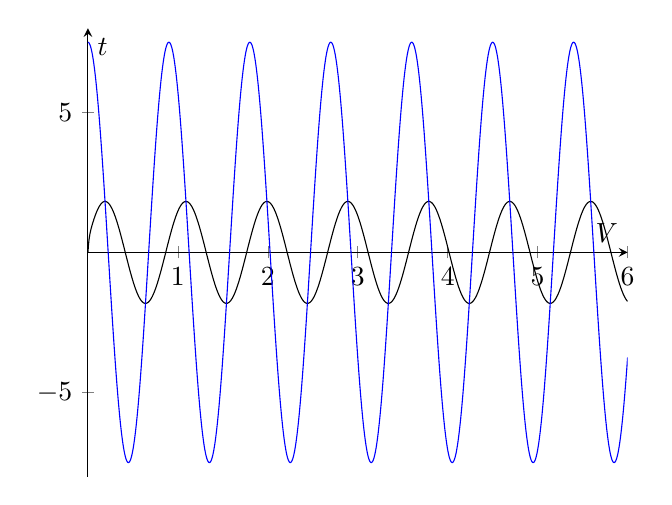
\begin{tikzpicture}[>=stealth]
    \begin{axis}[
        xmin=0,xmax=6,
        ymin=-8,ymax=8,
        axis x line=middle,
        axis y line=middle,
        axis line style=->,
        xlabel={$V$},
        ylabel={$t$},
        ]
				
        \addplot[no marks,black,-] expression[domain=0:6,samples=1000]
						{((7.5)/(sqrt(1 + 1000^2 * 0.00001^2 * 400^2))) * (((-2.718^((-x)/(1000*0.00001)))/(sqrt(1 + 1000^2 * 0.00001^2 * 400^2))) 
						+ cos(atan(-1000*0.00001*400) + 400*x))} 
						node[pos=0.65,anchor=south west]{$$};
						
				\addplot[no marks,blue,-] expression[domain=0:6,samples=1000]
						{7.5 * cos(400 * x)} 
						node[pos=0.65,anchor=south west]{$$}; 

    \end{axis}
	\end{tikzpicture}
	\caption{Graphe de $V_{out}$ (en noir) et $V_{in}$ (en bleu) pour les valeurs suivantes : $V_{max} = \unit{7.5}{\volt}$, $C = \unit{0.00001}{\farad}$,
						$R = \unit{1000}{\ohm}$ et $f = \unit{63.66}{\hertz}$}
	\label{lwp_voltages}
\end{figure}

\begin{figure}[!h]
	\centering
	\begin{tikzpicture}[>=stealth]
    \begin{axis}[
        xmin=0,xmax=1400,
        ymin=0,ymax=1.2,
        axis x line=middle,
        axis y line=middle,
        axis line style=->,
        xlabel={$f$},
        ylabel={$V_{out} / V_{in}$},
        ]
				
				\addplot[no marks,green,-] expression[domain=0:1400,samples=100]
						% Formule par rapport aux expressions obtenues, un peu décallée
						% {(((7.5)/(sqrt(1 + 100^2 * 0.00001^2 * (2*3.14*x)^2))) * (((-2.718^((-100*0.00001)/(100*0.00001)))/(sqrt(1 + 100^2 * 
						% 0.00001^2 * (2*3.14*x)^2))) + cos(atan(-100*0.00001*2*3.14*x) + 2*3.14*x*100*0.00001)))/(7.5 * cos(2*3.14*x*100*0.00001))}
						{(1 + (2*3.14*x*100*0.00001)^2)^(-0.5)}
						node[pos=0.65,anchor=south west]{$$}; 
    \end{axis}
	\end{tikzpicture}
	\caption{Graphe de $V_{out} / V_{in}$ pour les valeurs suivantes : $R = \unit{100}{\ohm}$ et $C = {\unit{0.0001}{\farad}}$.}
	\label{lwp_ratio}
\end{figure}

\bigbreak

\subsection{Le filtre passe-haut}

Soit $V_R$ la tension à travers la résistance $R$, $V_C$ la tension à travers
le condensateur $C$, $V_{in}$ la tension d'entrée et $V_{out}$ la tension de
sortie du filtre.

\begin{figure}[h]
	\centering
	\begin{circuitikz}
		\draw (0,0) node[ocirc] (A);
		\draw (0,0) to [C=$C$] (2,0);
		\draw (2,0) to [short] (4,0);
		\draw (4,0) node[ocirc] (C);
		\draw (2,0) to [R=$R$] (2,-2);
		\draw (2,-2) to [short] (4,-2);
		\draw (4,-2) node[ocirc] (D);
		\draw (0,-2) to [short] (2,-2);
		\draw (0,-2) node[ocirc] (B);
		\draw (A) to[open, v=$V_ {in}$] (B);
		\draw (C) to[open, v=$V_{out}$] (D);
	\end{circuitikz}
	\caption{Schéma électrique d'un filtre passe-haut.}
	\label{hgp_scheme}
\end{figure}

Sur la Figure \ref{hgp_scheme}, la loi des tensions de Kirchhoff donne la même équation que pour le filtre passe-bas :

$$V_{in} = V_R + V_C$$

Cette fois, $V_{out} = V_R$. Or on connait déjà $V_C$ que l'on a calculé dans
le section précédente. On a alors simplement :

$$V_R = V_{in} - V_C$$

$$V_{out} = V \cdot (\cos(\omega t) + \frac{e^{-\frac{t}{RC}}}{1 + R^2C^2\omega^2} - \frac{\cos(\arctan(-RC\omega) + \omega t))}{\sqrt(1 + R^2C^2\omega^2)})$$

Le déphasage reste donc le même que pour le filtre passe-bas.

\subsubsection{Vérification des résultats}

Pour le filtre passe-haut, on va cette fois vérifier que lorsque $\omega$ tend vers 0, on a
$V_{out}$ qui tend vers 0 également. Une fois de plus, c'est bien le cas.

On peut ensuite comparer les graphes de $V_{out}$, $V_{in}$ (Figure \ref{hgp_voltages}) et $V_{out} / V_{in}$
(Figure \ref{hgp_ratio}).

\begin{figure}[h]
	\centering
	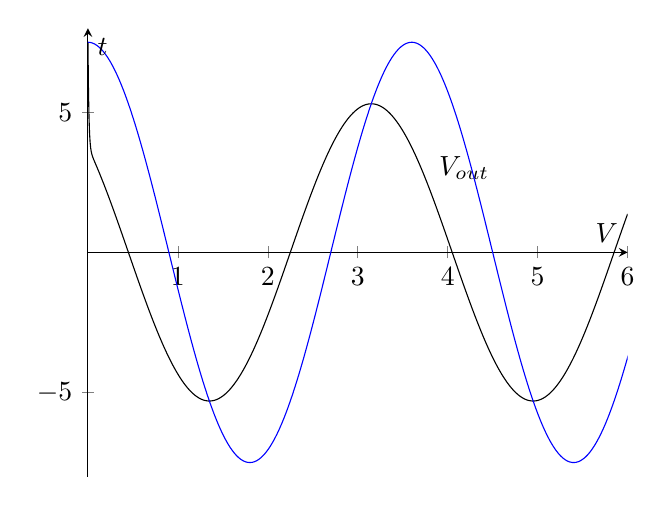
\begin{tikzpicture}[>=stealth]
    \begin{axis}[
        xmin=0,xmax=6,
        ymin=-8,ymax=8,
        axis x line=middle,
        axis y line=middle,
        axis line style=->,
        xlabel={$V$},
        ylabel={$t$},
        ]
				
        \addplot[no marks,black,-] expression[domain=0:6,samples=1000]
						{(7.5 * cos(100*x)) - ((7.5)/(sqrt(1 + 1000^2 * 0.00001^2 * 100^2))) * (((-2.718^((-x)/(1000*0.00001)))/(sqrt(1 + 1000^2 *
						0.00001^2 * 100^2))) + cos(atan(-1000*0.00001*100) + 100*x))} 
						node[pos=0.65,anchor=south west]{$V_{out}$};
						
				\addplot[no marks,blue,-] expression[domain=0:25,samples=1000]
						{7.5 * cos(100 * x)} 
						node[pos=0.65,anchor=south west]{$V_{in}$}; 
				
    \end{axis}
	\end{tikzpicture}
	\caption{Graphe de $V_{out}$ et $V_{in}$ pour les valeurs suivantes : $V_{max} = \unit{7.5}{\volt}$, $C = \unit{0.00001}{\farad}$,
					$R = \unit{1000}{\ohm}$ et $f = \unit{15.91}{\hertz}$}
	\label{hgp_voltages}
\end{figure}

\begin{figure}[h]
	\centering
	\begin{tikzpicture}[>=stealth]
    \begin{axis}[
        xmin=0,xmax=1400,
        ymin=0,ymax=1,
        axis x line=middle,
        axis y line=middle,
        axis line style=->,
        xlabel={$f$},
        ylabel={$V_{out}/V_{in}$},
        ]

				\addplot[no marks,green,-] expression[domain=0:1400,samples=100]
				% Formule obtenue avec nos expressions, décallée de 0.4 vers le haut.
				%		{((7.5 * cos(2*3.14*x*100*0.00001)) - ((7.5)/(sqrt(1 + 100^2 * 0.00001^2 * (2*3.14*x)^2))) * 		
				%	(((-2.718^((-100*0.00001)/(100*0.00001)))/(sqrt(1 + 100^2 *0.00001^2 * (2*3.14*x)^2))) + cos(atan(-100*0.00001*2*3.14*x) +
				%	2*3.14*x*100*0.00001)))/(7.5 * cos(2*3.14*x*100*0.00001))}
				{(1 + (1)/((2*3.14*x*100*0.00001)^2))^(-0.5)}
						node[pos=0.65,anchor=south west]{$$}; 

    \end{axis}
	\end{tikzpicture}
	\caption{Graphe de $V_{out} / V_{in}$ pour les valeurs suivantes : $R = \unit{100}{\ohm}$ et $C = {\unit{0.0001}{\farad}}$.}
	\label{hgp_ratio}
\end{figure}
Je peux modifier maintenant
\end{document}
